%!TEX root = principal.tex
\chapter{Programação - arduino}
O arduino é uma plataforma de microcontrolador simplificada. O nome arduino refere-se a: uma placa com um microcontrolador Atmel, uma linguagem de programação e um ambiente de desenvolvimento para esta linguagem. E também um auto-proclamado rei da Itália, mas este último não importa para nós.

A placa Arduino tem um conector USB para se ligar ao computador. Isto serve tanto para programar o microcontrolador quanto para comunicação entre os 2. Existem várias versões do arduino, pois já que é um sistema \emph{open-source} quem quiser pode fazer sua versão diferente da placa. Vamos nos referenciai aos arduinos UNO ou outras placas compatíveis com ele.

O arduino UNO tem 4 barras de pinos fêmeas para conexão com outros dispositivos: uma com tensões de alimentação (POWER), um com 6 entradas analógicas (ANALOG IN) e 2 com um total de 14 entradas e saídas digitais (DIGITAL).
\begin{figure}[hbt]
	\centering
	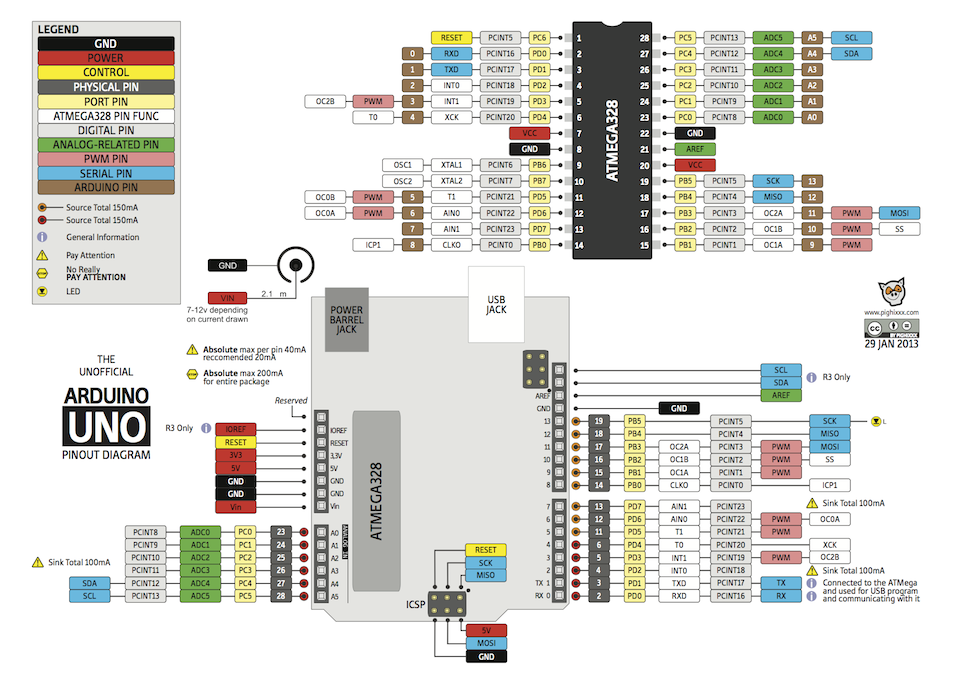
\includegraphics[width=\textwidth]{figuras/Arduino-Uno-Pinout}
	\caption{Pinagem do Arduino Uno}
	\label{fig:pinagem-arduino-uno}
\end{figure}

A linguagem de programação arduino é basicamente a linguagem C++ para microcontroladores ATMEL, mas com algumas funções e definições facilitadoras. A principal diferença entre C++ e a linguagem arduino é que não existe a função main(), mas sim as funções (ou rotinas) \lstinline|setup()| e \lstinline|loop()|. A função \lstinline|setup()| é executado apenas uma vez no momento que o arduino é ligado (ou resetado) e depois o código dentro da função \lstinline|loop()| é executado repetidamente. Com isto o esqueleto de um programa arduino fica:

\begin{lstlisting}[caption=Esqueleto de um programa arduino., label=lst:ardEsquel]
void setup() {
  //codigo a ser executado no inicio
}

void loop() {
  //codigo a ser executado repetidamente
}
 \end{lstlisting}

Lembrando que no arduino, como no C, tudo que tiver depois de \lstinline|//| é comentário e é ignorado pelo compilador.

\section{Piscando um led.}
Vamos passar logo a um exemplo para analisar um programa arduino. As placas de arduino UNO já tem um led ligado ao pino 13, identificado por um L na placa. Podemos fazer um programa que faça este led piscar.

\begin{lstlisting}[caption= Programa para piscar led.,label=lst:piscaled]
void setup() {
  //codigo a ser executado no inicio
  pinMode(13,OUTPUT); //define o pino 13 como uma saida (led)
}

void loop() {
  //codigo a ser executado repetidamente
  digitalWrite(13,LOW);  //apaga o led
  delay(500);            //espera meio segundo
  digitalWrite(13,HIGH); //acende o led
  delay(500);            //espera meio segundo
}	
\end{lstlisting}

A chamada \lstinline|pinMode(13, OUTPUT);| serve para definir que o pino 13 será uma saída. Obviamente isto só precisa ser feito no início do programa, logo está dentro de \lstinline|setup()|. Se quiséssemos ter uma entrada digital, usaríamos a mesma função, mas trocando OUTPUT por INPUT: \lstinline|pinMode(pino,INPUT);|.

A função que define o valor de um pino digital é a \lstinline|digitalWrite(pino,valor)|. Ela é chamada duas vezes no código \ref{lst:piscaled} dentro de \lstinline|loop()|, uma para apagar o led (gravando \lstinline|LOW|) e outra para acendê-lo (gravando \lstinline|HIGH|). \lstinline|LOW| e \lstinline|HIGH| são duas constantes, de valor 0 e 1, referentes ao zero e um lógico, respectivamente. Na prática, no sistema arduino, o \lstinline|LOW| é uma tensão próxima a \SI{0}{V} e o \lstinline|HIGH| uma tensão próxima a \SI{5}{V}.

Um detalhe é que o microcontrolador do arduino funciona numa velocidade de 8 ou \SI{16}{MHz} (dependendo da versão), logo se colocássemos apenas as duas chamadas à função \lstinline|digitalWrite| não veríamos o led piscar, mas teríamos a impressão que ele está aceso com metade da intensidade. Para vermos o led piscar é necessário colocar um atraso, que é justamente obtido pela função \lstinline|delay(x)|, que gera um tempo morto de \lstinline|x| milisegundos.

Se quiséssemos saber o valor de um pino digital que tivesse sido definido como entrada, a função seria \lstinline|digitalRead(pino)|, que retornaria o valor digital naquele pino. Pode-se usar isto por exemplo, para fazer com que uma saída digital seja a cópia de uma entrada digital, como no código \ref{lst:ardCopiaDig}.
\begin{lstlisting}[caption= Programa para acender um led em função de uma entrada digital.,label=lst:ardCopiaDig]
const int pinoSaida = 13;
const int pinoEntrada = 10;

int valor;

void setup() {
  //codigo a ser executado no inicio
  pinMode(pinoSaida,OUTPUT); //define a saida (led)
  pinMode(pinoEntrada,INPUT); //define a entrada
}

void loop() {
  //codigo a ser executado repetidamente
  valor = digitalRead(pinoEntrada); //le a entrada
  digitalWrite(pinoSaida,valor);  //e escreve na saida
}	
\end{lstlisting}

No código \ref{lst:ardCopiaDig} acrescentamos também algumas variáveis. Duas são constantes com os pinos usados. Elas facilitam a leitura do código e também facilitam caso posteriormente quisermos mudar os pinos utilizados. A outra variável armazena o valor lido da entrada, que depois é escrito na saída. 

%Altere o código do seu programa para que ele faça piscar um led ligado ao pino 5 do arduino.
\section{Sinais analógicos}
Em contraste com os sinais digitais, os sinais analógicos são aqueles que podem assumir qualquer valor de tensão. No contexto do arduino, vamos por enquanto assumir que os sinais analógicos estão entre \SI{0}{V} e \SI{5}{V}.

Para valores analógicos, usamos as funções \lstinline|analogWrite(pino,valor)| e \lstinline|analogRead(pino)|, que, ao contrário das equivalentes digitais, são restritas a alguns pinos específicos. As entradas analógicas são identificadas pelos pinos ANALOG IN (A0 a A5 no arduino) e são ligadas a um conversor analógico/digital (A/D) do microcontrolador, que transforma estes sinais numa palavra binária de 10 bits. Como $2^{10} = 1024$, isto significa que a função \lstinline|analogRead| retorna um valor entre 0 (para uma entrada de 0 V) e 1023 (para uma entrada de 5 V).

O arduino não tem um conversor D/A, logo a função \lstinline|analogWrite| não gera um sinal analógico verdadeiro no pino. O que esta função faz é gerar um sinal modulado por largura de pulso - PWM (\emph{Pulse Width Modulation}).

O sinal PWM é um trem de pulsos digital, com frequência da ordem de \SI{500}{Hz} (no caso do arduino) cuja razão entre o tempo em alto e o perído (conhecida como \emph{duty cycle}) pode ser alterada pelo parâmetro passado, como mostra a figura \ref{fig:pwm}.
\begin{figure}[hbt]
	\centering
	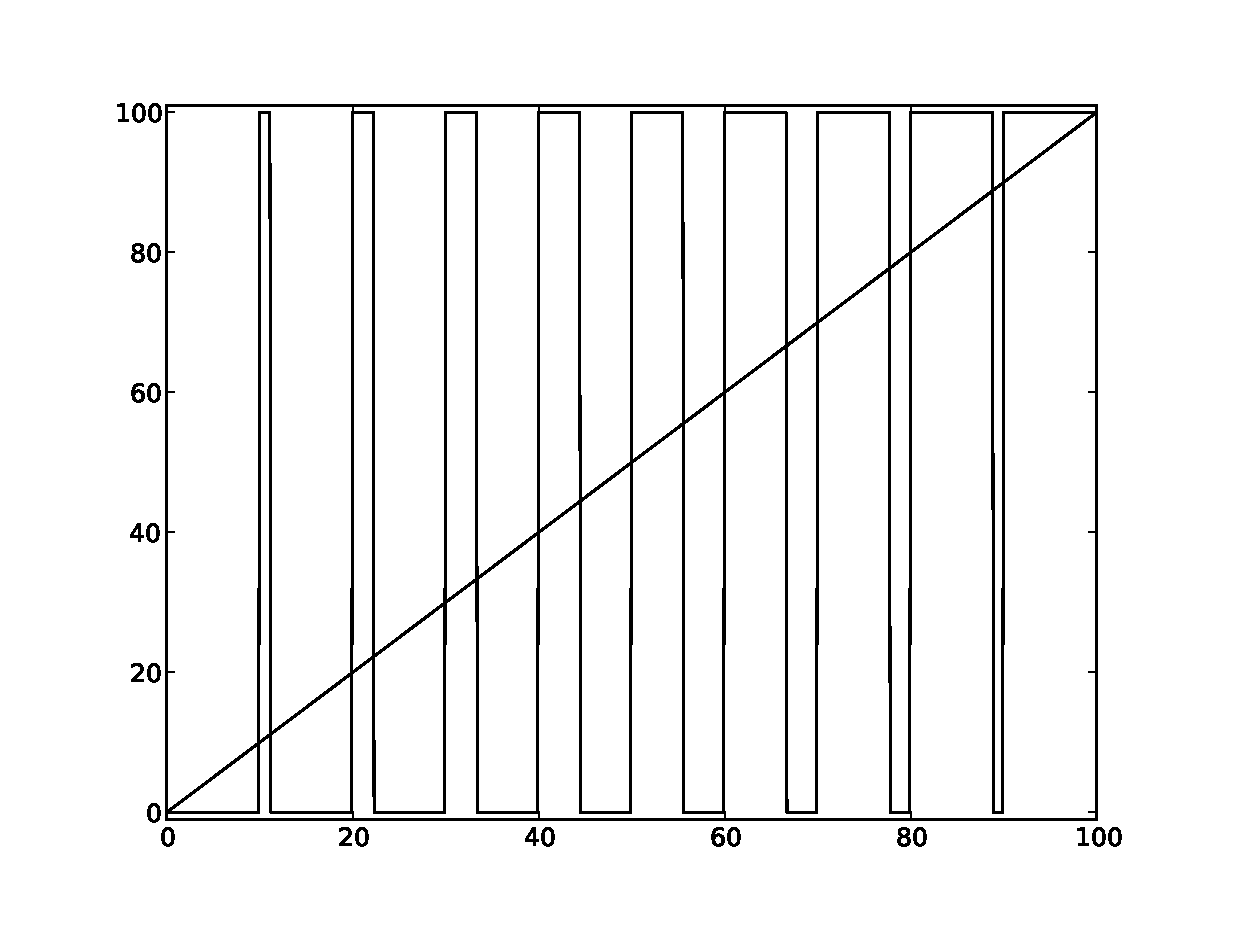
\includegraphics[width=\textwidth]{figuras/pwm}
	\caption{Reta modulada em largura de pulso (PWM).}
	\label{fig:pwm}
\end{figure}	
 Se um sinal PWM é enviado a um pino com um led, ele piscará 500 vezes por segundo, o que é muito rápido para o olho humano, de modo que na prática o que se vê quando se varia o duty cycle de um sinal PWM que aciona um led é uma variação de sua intensidade. Logo um sinal PWM funciona, para muitas aplicações, como um sinal analógico.

Novamente, não são todos os pinos do arduino que conseguem gerar este sinal PWM, logo a função \lstinline|analogWrite| está restrita aos pinos 3, 5, 6, 9, 10 e 11. Um outro detalhe que vale a pena ressaltar é que enquanto a função \lstinline|analogRead| gera um valor entre 0  1023, a \lstinline|analogWrite| recebe como parâmetro um valor entre 0 e 255 apenas.

Uma função útil do arduino para lidar com este tipo de situação é a função \lstinline|map(valor, minIn, maxIn, minOut, maxOut)|, que faz uma transformação linear de valor de acordo com a seguinte equação:
\begin{equation*}
(\text{valor} - \text{minIn}) \times \frac{\text{maxOut} - \text{minOut}}{\text{maxIn} - \text{minIn}} + \text{minOut}
\end{equation*}

A partir desta função, um código que leia o valor gerado pelo potenciômetro (em A0) e controle a intensidade do led no pino 5 poderia ser simplesmente:
\begin{lstlisting}
analogWrite(5,map(analogRead(A0),0,1024,0,256));
\end{lstlisting}

Note que o valor lido pelo \lstinline|analogRead| não precisa ser usado apenas na função \lstinline|analogWrite| mas pode ser usado para outra finalidade, como por exemplo alterar um atraso.
%Faça um programa que altere a frequência com que um led pisca em função da posição de um potênciometro.
%Repita o problema anterior, só que agora fazendo com que o led RGB ligado nos pinos 9, 10 e 11 pisque na sequencia vermelho, verde e azul, com a frequência definida pelo potenciômetro.
  
\section{Controle: for e if}
Até aqui foram feitos programas puramente sequenciais, porém em vários momentos é interessante realizar operações repetidas vezes ou realizar algumas tarefas apenas em situações específicas. Para estes casos existem comandos como o \lstinline|for| e o \lstinline|if|.
O comando for serve para tarefas repetidas. Por exemplo, se quiséssemos inicializar os pinos de 2 a 10 como saídas com valor LOW, poderíamos usar o seguinte código:
\begin{lstlisting}
for(int i = 2; i<11; i++){
	pinMode(i,OUTPUT);
	digitalWrite(i,LOW);
}	
\end{lstlisting}
O que este código faz é definir uma variável local i com valor inicial 2 depois ele checa se i é menor que 11, se for ele executa os comandos que estão entre as chaves ``\{'' e ``\}'', incrementa a variável \lstinline|i| (\lstinline|i++|) e checa novamente. Quando \lstinline|i < 11| for falso, ele sai do laço.

%Faça um programa que faça o led piscar suavemente (a intensidade variando entre apagado e totalmente aceso)
O comando if executa um determinado código apenas se determinada condição for verdadeira. Por exemplo, para acender um led apenas se um sinal analógico for maior que a metade da escala (512 = 1024/2)  pode-se escrever:
\begin{lstlisting}
if(analogRead(A0) >= 512){
	digitalWrite(13,HIGH);
}
\end{lstlisting}

Note que este código apenas fará alguma coisa se a condição for verdadeira. Para fazer uma coisa OU outra usa-se o comando \lstinline|else| após o \lstinline|if|:
\begin{lstlisting}
if(analogRead(A0) >= 512){
	digitalWrite(13,HIGH);
} else {
	digitalWrite(13,LOW);
}
\end{lstlisting}
%Faça o led rgb piscar suavemente em vermelho, azul ou verde dependendo do potenciômetro.
\section{Comunicação com o computador}
Como já dito, a conexão USB do arduino serve também para a comunicação do mesmo com o computador. Do lado do computador o arduino aparece como uma porta serial e o próprio programa contém um terminal serial pelo qual é possível se comunicar com o arduino. Do lado do arduino, os pinos 0 e 1 são os pinos transmissor e receptor ligados ao USB .

A programação é feita através do objeto  \lstinline|Serial|. Este objeto tem vários comandos, porém para nós os que interessam neste momento são:
\begin{description}
	\item[Serial.begin(baud)] Inicializa a comunicação serial na velocidade (baud rate) indicada.
	\item[Serial.read()] Retorna o valor de um byte recebido ou -1 caso não tenha sido recebido nenhum byte.
	\item[Serial.print(dado) e Serial.println(dado)] Se dado for um char ou uma string (texto), envia dado. Se dado for um número, envia este número como uma string. No caso de println, é acrescentada uma quebra de linha após dado.
	\item[Serial.available()] Retorna o número de bytes recebidos que ainda não foram lidos.
\end{description}

%Controle a intensidade das cores do led rgb pelo computador, enviando “cn” pela serial, onde 'c' é igual a 'r', 'g' ou 'b' e 'n' é um byte.
